W ostatnich latach sztuczna inteligencja i jej zastosowanie do przetwarzania obrazów zyskały na ogromnej popularności.
Jednym z wyzwań, jakie towarzyszą temu postępowi, jest problem detekcji obrazów zmodyfikowanych przez sztuczną inteligencję.
W dzisiejszych czasach, gdy coraz więcej osób wykorzystuje narzędzia do obróbki grafiki wykorzystujące metody inteligentne, łatwo jest zmienić oryginalne zdjęcie w sposób, który wygląda naturalny i trudny do wykrycia przez ludzkie oko.
Jednak, dzięki sztucznej inteligencji, możliwe jest wprowadzenie znacznie bardziej skomplikowanych i subtelnych modyfikacji, które są praktycznie niemożliwe do wykrycia przez człowieka.


Współczesna cyfrowa era zwiększyła zapotrzebowanie na wykrywanie obrazów zmodyfikowanych przez sztuczną inteligencję.
Wykrycie takich modyfikacji jest niezwykle ważne w wielu dziedzinach, takich jak obróbka obrazów medycznych, zabezpieczenia danych, bezpieczeństwo sieci, a także w badaniach naukowych.
Praca magisterska ta ma na celu przyczynienie się do rozwijania tej dziedziny wiedzy, poprzez wskazanie skutecznych metod detekcji i dostarczenie narzędzi umożliwiających wykrywanie obrazów zmodyfikowanych przez sztuczną inteligencję.


\section{Cel pracy}
Celem niniejszej pracy magisterskiej jest zbadanie i ocena skuteczności różnych metod detekcji obrazów zmodyfikowanych przez sztuczną inteligencję.
W ramach pracy zostaną przedstawione różne techniki i algorytmy służące do wykrywania modyfikacji obrazów, a także zostanie omówiona ich skuteczność w wykrywaniu modyfikacji wprowadzonych przez różne rodzaje sztucznej inteligencji.
Praca składać się będzie z teoretycznej części, gdzie omówione zostaną różne aspekty detekcji modyfikacji obrazów, oraz części praktycznej, gdzie zostaną przeprowadzone eksperymenty mające na celu porównanie skuteczności różnych metod detekcji.


\section{Aktualność wyboru tematu}
Wybór tematu dotyczącego detekcji obrazów zmodyfikowanych przez sztuczną inteligencję jest bardzo aktualny z kilku powodów.

Po pierwsze, sztuczna inteligencja i jej zastosowanie do przetwarzania obrazów rozwijają się bardzo szybko, a z tego wynikają różne wyzwania, w tym wyzwanie detekcji modyfikacji obrazów.
Zastosowanie sztucznej inteligencji w obróbce obrazów pozwala na wprowadzanie coraz bardziej skomplikowanych i subtelnych modyfikacji, które mogą być praktycznie niemożliwe do wykrycia przez człowieka.
Dlatego też jest coraz bardziej istotne, aby rozwijać metody i algorytmy pozwalające na wykrywanie takich modyfikacji.
Automatyczna detekcja obrazów wygenerowanych przez AI zaczyna pojawiać na największych portalach społecznościowych jak Twitter(przykład takiego powiadomienia pokazano na~\ref{img:twitter-notification})

\begin{wrapfigure}{r}{0.5\textwidth}
    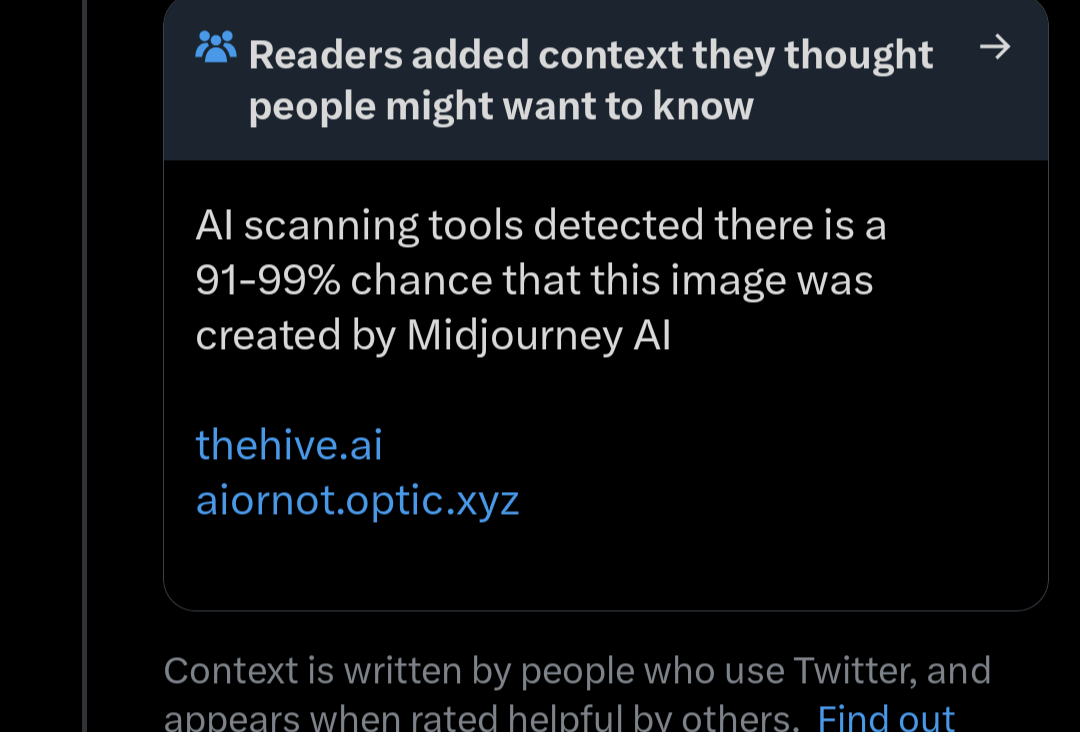
\includegraphics[width=\linewidth]{img/twitter}
    \centering
    \caption{ Powiadominie na portalu Twitter informujące o wykryciu obrazu wygenerowanego przez AI}
    \label{img:twitter-notification}
\end{wrapfigure}

Po drugie, zwiększone wykorzystanie narzędzi do obróbki obrazów, takich jak Photoshopm DeepFake cz Face2Face, sprawia, że łatwo jest zmienić oryginalne zdjęcie lub film w sposób, który wygląda naturalny i trudny do wykrycia przez ludzkie oko.
Tym samym, istnieje coraz większe zapotrzebowanie na narzędzia umożliwiające wykrywanie modyfikacji obrazów, aby zapobiegać oszustwom, np.
w kontekście fałszywych dokumentów, czy nieprawdziwych informacji w internecie.

\begin{wrapfigure}{l}{0.5\textwidth}
    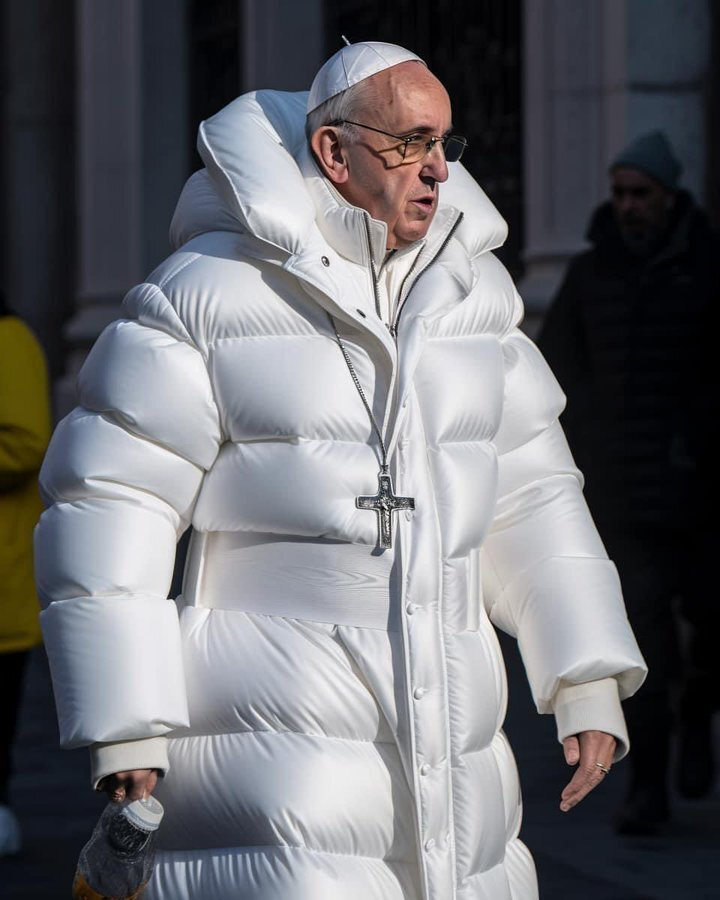
\includegraphics[width=\linewidth]{img/pope_balenciaga}
    \centering
    \caption{Wygenerowany obraz obraz znany jako "Balenciaga Pope".
    Przedstawiający papieża Franciszka noszącego kurtę wyglądającą na produkt dorgiej marki modowej Balenciaga.}
    \label{img:pope-balenciaga}
\end{wrapfigure}

Przykładem takiej kontrowersje jest obraz przedstawiający papieża Franciszka w drogiej puchowej kurtce (rysunek.~\ref{img:pope-balenciaga}).
Papież Franciszek, który jest głową Kościoła katolickiego, nie jest znany z ostentacyjnego stylu życia ani noszenia drogich ubrań.
W związku z tym, informacje sugerujące, że papież był widziany w drogiej kurtce puchowej Balenciaga, wywołały pewien skandal.
Szybko zauważono artefakty występujące na obrazie i co za tym idzie fakt że został wygenerowany przez AI. Artefakty tym na obrazie zostały omówione w rozdziale~\ref{sec:section-artifacts}.
Ten mini-skandal był jedną z przyczyn szybkiego wprowadzenia przez Twittera wspomnianych wcześniej komunikatów o obrazach wygenerowanych przez AI, pokazanych na rysunku~\ref{img:twitter-notification}.


Wreszcie, detekcja modyfikacji obrazów jest istotna w wielu dziedzinach, takich jak obróbka obrazów medycznych, zabezpieczenia danych, bezpieczeństwo sieci czy badania naukowe.
W związku z tym, rozwój metod i algorytmów umożliwiających wykrywanie modyfikacji jest bardzo istotny dla postępu w tych dziedzinach.


Podsumowując, wybór tematu dotyczącego detekcji obrazów zmodyfikowanych przez sztuczną inteligencję jest bardzo aktualny, ponieważ rozwój sztucznej inteligencji i narzędzi do obróbki obrazów, wraz z rosnącym zapotrzebowaniem na wykrywanie modyfikacji, sprawiają, że rozwijanie metod i algorytmów w tym zakresie jest niezwykle ważne.